% !TeX program = latexmk
% !TeX options = -xelatex -synctex=1 -interaction=nonstopmode -file-line-error -outdir=build "%DOC%"
% =============================================================================
% 数学建模竞赛论文通用 LaTeX 模板
% =============================================================================
\documentclass[12pt,a4paper,fontset=windows]{ctexart}

% ============================ 1. 宏包加载 ====================================
\usepackage{geometry}
\geometry{left=2.5cm, right=2.5cm, top=2.5cm, bottom=2.5cm}

\usepackage{amsmath, amssymb}
\usepackage{booktabs}
\usepackage{multirow}
\usepackage{array}
\usepackage{makecell}
\usepackage{graphicx}
\usepackage{float}
\usepackage{fancyhdr}
\usepackage{indentfirst}
\usepackage{caption}
\usepackage{subcaption}
\usepackage{longtable}
\usepackage{listings}
\usepackage{xcolor}
\usepackage{enumitem}
\usepackage{hyperref}

\usepackage{tikz}
\usetikzlibrary{shapes.geometric, arrows.meta, positioning, calc, fit, backgrounds}

% ============================ 2. 字体设置 ====================================

% ============================ 3. 超链接设置 ==================================
\hypersetup{
    colorlinks=true,
    linkcolor=black,
    citecolor=black,
    urlcolor=blue,
    bookmarksopen=true,
    pdftitle={微构体中填充导电介质的仿真优化},
    pdfauthor={参赛队}
}

% ============================ 4. 代码块设置 ==================================
\lstset{
    language=Python,
    basicstyle=\small\ttfamily,
    keywordstyle=\color{blue},
    commentstyle=\color{green!60!black},
    stringstyle=\color{red!70!black},
    numbers=left,
    numberstyle=\tiny\color{gray},
    frame=single,
    breaklines=true,
    tabsize=4,
    showstringspaces=false,
    literate={_}{{\_}}1,
    captionpos=b
}

% ============================ 5. 章节标题格式 ================================
\ctexset{
    section/name={,},
    section/number=\chinese{section}、,
    section/format=\large\bfseries\centering,
    subsection/number=\arabic{subsection},
    subsection/format=\bfseries,
    subsubsection/number=\arabic{subsection}.\arabic{subsubsection},
    subsubsection/format=\itshape
}

% ============================ 6. 正文排版间距 ================================
\renewcommand{\baselinestretch}{1.5}
\setlength{\parskip}{0.5em}
\setlength{\parindent}{2em}

\captionsetup{justification=centering}
\captionsetup[table]{position=above}
\captionsetup[figure]{position=below}

\setlist{nosep, leftmargin=2em}

% ============================ 7. 页眉页脚 ====================================
\pagestyle{fancy}
\fancyhf{}
\fancyfoot[C]{\thepage}
\renewcommand{\headrulewidth}{0pt}

% ============================ 8. 自定义命令 ==================================
\newcommand{\abstractpage}[3]{%
    \thispagestyle{plain}%
    \pagenumbering{arabic}%
    \setcounter{page}{1}%
    \begin{center}
        {\bfseries\zihao{3} #1}%
    \end{center}
    \vspace{0.5em}
    \begin{center}
        {\bfseries\zihao{4} 摘\quad 要}%
    \end{center}
    \vspace{0.5em}
    #2%
    \vspace{1em}
    \par\noindent\textbf{关键词}：#3
    \newpage
}

\newcommand{\res}[1]{\textbf{#1}}
\newcommand{\nm}{\,\mathrm{nm}}
\newcommand{\um}{\,\mu\mathrm{m}}

% =============================================================================
\begin{document}

\abstractpage{微构体中填充导电介质的仿真优化}%
{%
针对边长 $10000\nm$ 微构体中导电介质填充与跨电极导通问题，本文建立以几何连通图为基础、蒙特卡洛仿真为核心、成本优化为目标的统一建模框架：问题一判断附件构型的确定性导通状态，问题二估计不同体积分数下的导通概率，问题三搜索满足 90\% 概率阈值的最低填充量，问题四以最小成本为目标进行 A/B 混合优化。

针对问题一，读取附件三组 A 介质端点坐标，恢复圆柱轴线并以最小镜像距离处理周期边界，构造介质—电极连通图。结果表明：组 1 含 12 根 A 不导通，组 2 含 49 根 A 导通，组 3 含 535 根 A 导通，说明"总填充量"不是导通的唯一指标，介质位置与取向同样关键。

针对问题二，将四个体积分数换算为 $354$、$424$、$495$、$707$ 根 A，各进行 $4000$ 次蒙特卡洛试验，采用 Wilson 区间估计概率。结果显示：$\phi_A=0.50\%$ 时 $\hat p=0.0748$，$0.60\%$ 时 $0.2035$，$0.70\%$ 时 $0.4520$，$1.00\%$ 时 $0.9845$，概率随填充量单调上升，呈典型渗流型曲线。

针对问题三，采用粗网格扫描与二分搜索相结合的策略，以 Wilson 下限作为统计认证标准，得到最低认证体积分数约为 $0.87\%$，对应约 $615$ 根 A。

针对问题四，构建 A/B 混合成本模型，A 单位体积价格约为 B 的 $21$ 倍。网格搜索表明：$580$ 根 A 与 $115$ 个 B 组合概率 $0.9140$、成本 $8.9876$ 元；$283$ 根 A 与 $119$ 个 B 组合概率 $0.917$、成本 $4.4002$ 元，体现长圆柱骨架与低价球体的互补作用。

综上，本文通过周期边界最小镜像距离、并查集与 BFS 连通判定、蒙特卡洛概率估计及网格搜索成本优化，建立了完整的微构体导电仿真框架，可推广至更复杂的介质分布与导通判据。
}%
{微构体；周期边界；随机几何图；蒙特卡洛；成本优化}

% ============================================================================
% 一、问题重述
% ============================================================================
\section{问题重述}

导电复合体系通常由导电颗粒、导电纤维或连续相共同承担电荷传输功能。在微观尺度，宏观的"导通"并不要求所有介质相互接触，而只要求存在一条从一个电极到另一个电极的连续或近连续路径。题目将实际材料理想化为边长 $10000\nm$ 的立方体，将两相对表面设为带电面，并规定导电介质之间的间隙阈值为 $1.8\nm$。这种设定把物理过程转化为具有明确几何规则的随机连通问题。

本研究关注三个相互衔接的层次。第一层次是确定性几何判断，即附件给出的三组介质 A 端点坐标是否已经形成跨越 $X$ 方向的路径。第二层次是随机填充下的概率规律，即给定 A 的体积分数后，重复随机生成微构体并统计导通比例。第三层次是工程设计，即在导通概率达到 90\% 的前提下，寻找最小单一填充量或最低混合成本。

问题一要求读取附件三个分表，依据圆柱端点坐标恢复每根 A 的轴线，判断三组微构体是否导通。问题二要求只填充 A，研究四个指定体积分数的导通概率。问题三要求在概率不低于 90\% 的约束下寻找 A 的最低体积分数。问题四同时考虑 A 与 B，并把 A、B 的单位体积成本纳入目标函数。

\begin{table}[H]\centering\caption{题目输入、输出与评价指标}\begin{tabular}{p{2.5cm}p{4.2cm}p{4.2cm}p{3cm}}\toprule 子问题&主要输入&主要输出&评价指标\\\midrule 问题一&三组端点坐标&导通/不导通、路径&连通性\\问题二&A体积分数&概率估计、区间&概率与抽样误差\\问题三&A数量搜索&最低体积分数&概率阈值\\问题四&A/B数量、成本&混合方案&成本与概率\\\bottomrule\end{tabular}\end{table}

% ============================================================================
% 二、问题分析
% ============================================================================
\section{问题分析}

\subsection{附件结构与数据审计}
附件 Excel 包含三个工作表。每个工作表前两行为表头，之后每行对应一根介质 A，前三列是第一个端点坐标，后三列是另一个端点坐标。程序逐行读取数值并转换为浮点型数组，不对坐标进行人工平移，因此保留了题目给出的边界端点。

\begin{table}[H]\centering\caption{附件工作表规模检查}\begin{tabular}{cccccc}\toprule 工作表&有效数据行&坐标列&最小坐标&最大坐标&异常值\\\midrule 组1&12&6&-5000&5000&无\\组2&49&6&-5000&5000&无\\组3&535&6&-5000&5000&无\\\bottomrule\end{tabular}\end{table}

图~\ref{fig:q1_counts} 显示三组介质数量相差明显，第三组已经接近高密度网络，因而不能用同一个固定的邻接数量近似所有构型。

\begin{figure}[H]\centering
\includegraphics[width=.72\textwidth]{figures/fig_q1_counts.pdf}\caption{附件三组介质 A 数量}\label{fig:q1_counts}\end{figure}

\subsection{体积换算}
圆柱 A 的体积为 $V_A=\pi r^2h$，球 B 的体积为 $V_B=4\pi R^3/3$。代入题面尺寸得到 $V_A=1.4137167\times 10^7\nm^3$、$V_B=3.3510322\times10^7\nm^3$。立方体体积为 $10^{12}\nm^3$，因此每个 A 约占 $0.0014137\%$，每个 B 约占 $0.0033510\%$。数量取整会造成不超过半个单体体积的舍入误差，远小于本文体积分数网格间隔。

\begin{table}[H]\centering\caption{几何与物理参数}\begin{tabular}{llll}\toprule 参数&符号&数值&单位\\\midrule 立方体边长&$L$&10000&nm\\A半径&$r$&30&nm\\A高度&$h$&5000&nm\\B半径&$R$&200&nm\\导通间隙&$d_0$&1.8&nm\\A单体体积&$V_A$&$1.4137167\times10^7$&nm$^3$\\B单体体积&$V_B$&$3.3510322\times10^7$&nm$^3$\\\bottomrule\end{tabular}\end{table}

\subsection{周期边界解释}
题目的边界截断规则要求越界部分沿对应方向平移一个边长重新进入立方体。若把所有平移后的副本同时看作一个周期空间，则任意两个实体的真实最近距离就是所有整数平移副本距离的最小值。由于边长远大于介质半径，实际计算只需检查最近镜像，即对位移 $\Delta$ 使用
\begin{equation}\Delta^*=\Delta-L\operatorname{round}(\Delta/L)。\end{equation}
该处理同时适用于 A--A、A--B 和 B--B 的距离。

\subsection{研究技术路线}
本文的技术路线如图~\ref{fig:workflow} 所示。首先对 PDF 题面和 Excel 附件进行数据审计；然后把边界规则转化为最小镜像距离；再构造连通图；最后以蒙特卡洛仿真和网格搜索完成概率、阈值与成本优化。每一阶段都保存中间数据，确保论文中的数字可以追溯到程序输出。
\begin{figure}[H]\centering
\begin{tikzpicture}[>=stealth, thick]

\tikzset{
    mybox/.style={rectangle, rounded corners=4pt, minimum width=2.3cm, minimum height=0.78cm,
                  text centered, font=\small\bfseries, line width=0.5pt,
                  top color=#1!20!white, bottom color=#1!6!white, draw=#1!55!black},
    mylabel/.style={rectangle, rounded corners=2pt, minimum height=0.32cm, text centered,
                    font=\scriptsize\bfseries, text=white, fill=#1!65!black, inner sep=2pt}
}

% ── 标签 ──
\node[mylabel=blue]   at (0, 2.15)   {数据准备};


% ── 第一行 ──
\node[mybox=blue]   (B1) at (0, 1.5)   {附件读取};
\node[mybox=cyan]   (B2) at (3.5, 1.5)  {\shortstack{周期边界\\[-1pt]\scriptsize 最小镜像}};
\node[mybox=teal]   (B3) at (7.0, 1.5)  {\shortstack{胶囊体距离\\[-1pt]\scriptsize 线段最近点}};
\node[mybox=green]  (B4) at (10.5, 1.5) {\shortstack{连通图构建\\[-1pt]\scriptsize 并查集}};

\draw[->, line width=0.6pt, color=blue!50!black]   (B1) -- (B2);
\draw[->, line width=0.6pt, color=cyan!50!black]   (B2) -- (B3);
\draw[->, line width=0.6pt, color=teal!50!black]   (B3) -- (B4);

% ── 第二行 ──
\node[mybox=orange] (B5) at (0, -1.0)   {\shortstack{蒙特卡洛\\[-1pt]\scriptsize 随机生成}};
\node[mybox=red]    (B6) at (3.5, -1.0)  {\shortstack{阈值搜索\\[-1pt]\scriptsize Wilson 认证}};
\node[mybox=purple] (B7) at (7.0, -1.0)  {\shortstack{成本优化\\[-1pt]\scriptsize A/B 混合}};
\node[mybox=gray]   (B8) at (10.5, -1.0) {\shortstack{论文输出\\[-1pt]\scriptsize 图表生成}};

\draw[->, line width=0.6pt, color=orange!50!black] (B5) -- (B6);
\draw[->, line width=0.6pt, color=red!50!black]    (B6) -- (B7);
\draw[->, line width=0.6pt, color=purple!50!black] (B7) -- (B8);

% ── 跨行箭头 ──
\draw[->, line width=0.6pt, color=green!60!black, dashed]
    (B4.south) -- ++(0,-0.35) -| (B5.north);

\end{tikzpicture}
\caption{总体技术路线}\label{fig:workflow}
\end{figure}

% ============================================================================
% 三、模型假设
% ============================================================================
\section{模型假设}

为使题面规则可计算，作出以下假设：
\begin{enumerate}[label=(\arabic*)]
\item 介质位置在立方体内均匀独立生成，介质之间允许重叠；
\item A 的轴向方向服从球面均匀分布，长度固定为 $h$，半径固定为 $r$；
\item B 为理想球体，半径固定为 $R$，不考虑形变；
\item 两个实体的最短表面间隙不超过 $d_0$ 即可导通，导通不随时间衰减；
\item 左右带电面是理想电极，其余四面绝缘，仅用于周期边界回绕；
\item 概率估计中的随机数流固定，以保证不同运行之间可比较。
\end{enumerate}
每条假设都对应一个可检验的替代方案。例如，将独立均匀位置改为排斥采样会降低局部团聚；将固定方向改为偏向 $X$ 轴会提高跨面概率。本文在模型评价与推广一节讨论这些扩展。

% ============================================================================
% 四、符号说明
% ============================================================================
\section{符号说明}

\begin{longtable}{p{2.2cm}p{7cm}p{3cm}}\caption{主要符号}\\\toprule 符号&含义&单位\\\midrule\endhead $L$&微构体边长&nm\\ $r,h$&A半径与高度&nm\\ $R$&B半径&nm\\ $d_0$&导通间隙阈值&nm\\ $S_i$&第$i$根A轴线线段&nm\\ $c_j$&第$j$个B球心&nm\\ $N_A,N_B$&A、B数量&个\\ $\phi_A,\phi_B$&A、B体积分数&\%\\ $I_k$&第$k$次试验的导通指示变量&0/1\\ $\hat p$&导通概率估计&无量纲\\ $C$&总填充成本&元\\\bottomrule\end{longtable}

令 $G=(V,E)$ 为无向图，节点集合包括所有介质节点和两个电极节点 $L_e,R_e$。若两个介质满足实体距离准则，则在 $E$ 中加入边；若介质与某电极面满足面距离准则，则加入介质--电极边。微构体导通当且仅当 $L_e$ 与 $R_e$ 在 $G$ 中连通。该定义把极化作用纳入图的传递闭包：一旦一个节点与带电分量相连，整个分量均视为带电。

% ============================================================================
% 五、模型的建立与求解
% ============================================================================
\section{模型的建立与求解}

\subsection{问题一：附件构型的确定性判定}

\subsubsection{轴线恢复}
附件每行两个端点 $p_i,q_i\in\mathbb{R}^3$ 正好给出圆柱 $A_i$ 轴线与两个底面中心的交点。轴向长度 $\|q_i-p_i\|$ 应接近题设高度 $h=5000\nm$。程序对所有行检查该长度，并在后续距离计算中直接使用线段 $S_i=[p_i,q_i]$ 表征圆柱的中心轴，避免用端点欧氏距离替代实体间最短距离。

\subsubsection{胶囊体距离模型}
题目中圆柱 A 的两端为半球形封盖，整体构成一个胶囊体（capsule），即半径为 $r$ 的球沿轴线 $S_i$ 扫掠形成的几何体。同理，球 B 可视为退化的胶囊体（轴线长度为零）。两个胶囊体之间的最短间隙等价于它们各自中心轴线之间的最短距离再减去两者的半径：
\begin{equation}
d_{\mathrm{gap}}(A_i,A_j) = d_{\mathrm{seg}}(S_i,S_j) - r_A - r_A,
\label{eq:cap_aa}
\end{equation}
\begin{equation}
d_{\mathrm{gap}}(A_i,B_j) = d_{\mathrm{seg}}(S_i,\{c_j\}) - r_A - r_B,
\label{eq:cap_ab}
\end{equation}
\begin{equation}
d_{\mathrm{gap}}(B_i,B_j) = \|c_i^*-c_j\| - 2r_B,
\label{eq:cap_bb}
\end{equation}
其中 $d_{\mathrm{seg}}$ 表示两线段之间的最短欧氏距离，$c_j$ 为球心坐标，$c_i^*$ 表示经过周期镜像平移后的球心。当 $d_{\mathrm{gap}}\le d_0=1.8\nm$ 时判定两介质导通。

\subsubsection{两线段最短距离的参数化求解}
设线段 $S_i=[p_i,q_i]$ 和 $S_j=[p_j,q_j]$，令 $u=q_i-p_i$、$v=q_j-p_j$、$w=p_i-p_j$。$S_i$ 上的任意点可参数化为 $a(s)=p_i+su$，$S_j$ 上的任意点为 $b(t)=p_j+tv$，其中 $s,t\in[0,1]$。两线段间最短距离等价于
\begin{equation}
\min_{s,t\in[0,1]} f(s,t)=\|w+su-tv\|^2.
\label{eq:segmin}
\end{equation}
展开 $f(s,t)$ 得
\begin{equation}
f(s,t)=aa\cdot s^2 - 2b\cdot st + c\cdot t^2 + 2d\cdot s - 2e\cdot t + \|w\|^2,
\label{eq:segexpand}
\end{equation}
其中各内积系数为
\begin{equation}
aa=u^\top u,\quad c=v^\top v,\quad b=u^\top v,\quad d=u^\top w,\quad e=v^\top w.
\end{equation}

令偏导数为零求无约束极值点：
\begin{equation}
\frac{\partial f}{\partial s}=2(aa\cdot s - b\cdot t + d)=0,\qquad
\frac{\partial f}{\partial t}=2(-b\cdot s + c\cdot t - e)=0.
\end{equation}
写成矩阵形式
\begin{equation}
\begin{pmatrix}aa & -b \\ -b & c\end{pmatrix}\begin{pmatrix}s \\ t\end{pmatrix}=\begin{pmatrix}-d \\ e\end{pmatrix},
\label{eq:seglinear}
\end{equation}
当行列式 $\Delta=aa\cdot c - b^2 > 0$（即两线段不平行）时，无约束最优解为
\begin{equation}
s^*=\frac{be-cd}{\Delta},\qquad t^*=\frac{bs^*+e}{c}.
\label{eq:seg_analytic}
\end{equation}

由于 $s,t$ 必须限制在 $[0,1]$ 内，实际求解采用\textbf{先内后外}的策略：
\begin{enumerate}[label=(\roman*)]
\item 若 $s^*\in[0,1]$，直接代入求 $t_{\mathrm{nom}}=bs^*+e$；
\item 若 $t_{\mathrm{nom}}\in[0,c]$（即 $t^*=t_{\mathrm{nom}}/c\in[0,1]$），则 $(s^*,t^*)$ 为内部最优解；
\item 否则将 $t$ 投影到边界 $t=0$ 或 $t=1$，再在对应边界上对 $s$ 求一维最优：
\begin{equation}
t=0 \Rightarrow s=\mathrm{clip}(-d/aa,\,0,\,1); \qquad
t=1 \Rightarrow s=\mathrm{clip}((b-d)/aa,\,0,\,1).
\end{equation}
\end{enumerate}
最终两线段最短距离为
\begin{equation}
d_{\mathrm{seg}}(S_i,S_j)=\left\|w+s^*u-t^*v\right\|.
\label{eq:segresult}
\end{equation}

\subsubsection{周期边界的最小镜像处理}
立方体具有周期边界：介质超出 $[-L/2,L/2]^3$ 的部分沿对应方向平移一个边长 $L$ 后重新进入立方体。对任意位移向量 $\Delta$，最近镜像位移为
\begin{equation}
\Delta^*=\Delta - L\left\lfloor\frac{\Delta}{L}+\frac{1}{2}\right\rfloor = \Delta - L\cdot\mathrm{round}(\Delta/L),
\label{eq:minimage}
\end{equation}
其中 $\lfloor\cdot\rfloor$ 为向下取整，$\mathrm{round}(\cdot)$ 为四舍五入。该式将每个分量映射到 $[-L/2,L/2]$ 范围内。

在胶囊体距离计算中，最小镜像应用于第二个对象的中心：先计算两对象中心的位移 $\Delta$，取 $\Delta^*$ 后将第二个对象整体平移 $\Delta^*$，再在平移后的坐标上执行线段距离或球心距离计算。对线段 $S_j=[p_j,q_j]$ 的具体操作为
\begin{equation}
p_j^*=p_j+\Delta^*,\qquad q_j^*=q_j+\Delta^*.
\label{eq:segshift}
\end{equation}

\subsubsection{介质—电极面距离}
左电极面为 $x=-L/2$，右电极面为 $x=+L/2$。介质 $A_i$ 的端点 $p_i$ 到某电极面的最短距离需考虑周期边界：端点可能因越界而被截断到对面。对端点 $p_i$ 的 $x$ 坐标 $x_i$，到面 $x=f$ 的距离为
\begin{equation}
d_{\mathrm{face}}(p_i,f)=\min_{k\in\{-1,0,1\}}|x_i+kL-f|.
\label{eq:face_dist}
\end{equation}
对于线段（而非单个端点），还需检查线段是否穿越立方体边界后被截断到另一侧。程序将线段按 $x=\pm L/2$ 处的交叉点分割为若干子段，对每个子段独立判断其所属的周期镜像，再取各子段到电极面距离的最小值。当线段穿越电极面时距离为零。

导通判定中，若 $\min(d_{\mathrm{face}}(p_i,-L/2),\,d_{\mathrm{face}}(q_i,-L/2))\le d_0$，则 $A_i$ 与左电极导通；右电极同理。

\subsubsection{连通图构建}
以所有介质（$N_A$ 根圆柱 + $N_B$ 个球）和左右两个电极共 $N_A+N_B+2$ 个节点构建无向图 $G=(V,E)$。边的判定准则为：
\begin{itemize}
\item \textbf{A--A 边}：若 $d_{\mathrm{gap}}(A_i,A_j)\le d_0$，加入边 $(i,j)$；
\item \textbf{A--B 边}：若 $d_{\mathrm{gap}}(A_i,B_j)\le d_0$，加入边 $(i,j)$；
\item \textbf{B--B 边}：若 $d_{\mathrm{gap}}(B_i,B_j)\le d_0$，加入边 $(i,j)$；
\item \textbf{A--电极边}：若 $A_i$ 到某电极面距离 $\le d_0$，加入介质到电极的边。
\end{itemize}
微构体导通当且仅当左电极节点与右电极节点在 $G$ 中连通。使用并查集（Disjoint Set Union）维护连通分量，所有边扫描完成后仅需一次根节点比较即可判定导通。

\subsubsection{判定结果}
三组的结果列于表~\ref{tab:q1result}。图~\ref{fig:q1geometry} 是组1在 $X-Y$ 平面的端点投影，虚线为两个带电面。
\begin{table}[H]\centering\caption{问题一确定性计算结果}\label{tab:q1result}\begin{tabular}{ccccc}\toprule 组别&A数量&左面连接节点&右面连接节点&导通\\\midrule 1&12&0&0&否\\2&49&1&1&是\\3&535&多节点&多节点&是\\\bottomrule\end{tabular}\end{table}
\begin{figure}[H]\centering
\includegraphics[width=.85\textwidth]{figures/fig_q1_geometry.pdf}\caption{组1介质 A 的几何投影}\label{fig:q1geometry}\end{figure}

\subsubsection{路径解释}
组1仅有 12 根圆柱，数量过少且分布分散，未形成从左电极到右电极的完整路径；组2含 49 根圆柱，其中少数几何上恰好接近两个电极的长圆柱通过中间节点完成跨越；组3含 535 根圆柱，节点密度足够高，连通分量显著增大。该结果说明"总填充量"不是确定性导通的唯一指标，介质位置和取向同样关键。

\subsection{问题二：A 单填充的蒙特卡洛模型}

\subsubsection{渗流理论背景}
导电介质在绝缘基体中的随机分布可抽象为连续渗流模型\cite{berhan2007}。对于高长径比纤维（如本题中的圆柱 A），渗流阈值 $\phi_c$ 与排除体积 $V_{\mathrm{ex}}$ 之间存在反比关系：
\begin{equation}
\phi_c \approx \frac{1}{n_c V_{\mathrm{ex}}},
\label{eq:percolation_threshold}
\end{equation}
其中 $n_c$ 为临界数密度，$V_{\mathrm{ex}}$ 为两根纤维在任意相对位置和取向下可能重叠的平均排除体积。对于长径比 $\kappa=h/(2r)$ 的圆柱体，排除体积为\cite{berhan2007}
\begin{equation}
V_{\mathrm{ex}} = 2\pi r^2 h + \frac{4}{3}\pi(2r)^3 = 2\pi r^2 h + \frac{32}{3}\pi r^3,
\label{eq:excluded_volume}
\end{equation}
其中第一项为两平行圆柱的排除体积主导项，第二项为端部半球的修正。对于本题参数（$r=30\nm$，$h=5000\nm$，$\kappa\approx 83$），$V_{\mathrm{ex}}\approx 3.40\times10^7\nm^3$，远大于单个圆柱体积 $V_A=1.41\times10^7\nm^3$，说明高长径比介质在极低体积分数下即可形成渗流网络。

在渗流阈值附近，导通概率 $\Pi(\phi)$ 遵循标度律\cite{ziff2002}：
\begin{equation}
\Pi(\phi) \sim (\phi - \phi_c)^t, \qquad \phi \to \phi_c^+,
\label{eq:scaling_law}
\end{equation}
其中 $t$ 为渗流临界指数，在三维系统中 $t\approx 2.0$。这意味着概率曲线在阈值附近呈现急剧上升的 S 形特征，与本题数值结果一致。

\subsubsection{随机构型生成}
每次试验先生成中心 $z_i\sim U([-L/2,L/2]^3)$，再生成三维正态向量 $g_i$ 并归一化为单位方向 $u_i=g_i/\|g_i\|$。A 的两个端点为 $z_i\pm hu_i/2$。这种方法产生球面均匀方向，不会偏向任一坐标轴。每个构型等价于从位置-取向联合空间中的一次均匀抽样，确保蒙特卡洛估计的无偏性。

\subsubsection{概率估计与置信区间}
对固定数量 $N_A$ 重复 $M$ 次独立试验，记导通次数为 $K$，则导通概率的极大似然估计为 $\hat p=K/M$。由于 $\hat p$ 服从二项分布 $B(M,p)/M$，其方差为 $p(1-p)/M$。

经典的 Wald 区间 $\hat p\pm z\sqrt{\hat p(1-\hat p)/M}$ 在 $p$ 接近 0 或 1 时覆盖率严重偏离标称水平\cite{brown2001}。本文采用 Wilson 分数区间，其构造基于对二项分布参数 $p$ 的 Score 检验统计量：
\begin{equation}
CI_W = \left[\frac{\hat p + \frac{z^2}{2M} - \frac{z}{2M}\sqrt{4M\hat p(1-\hat p)+z^2}}{1+z^2/M},\;
\frac{\hat p + \frac{z^2}{2M} + \frac{z}{2M}\sqrt{4M\hat p(1-\hat p)+z^2}}{1+z^2/M}\right],
\label{eq:wilson}
\end{equation}
其中 $z=z_{\alpha/2}$ 为标准正态分位数（95\% 置信度下 $z=1.96$）。Wilson 区间的优势在于\cite{brown2001}：(i) 当 $K=0$ 或 $K=M$ 时下界严格大于 0 或上界严格小于 1，避免了 Wald 区间退化为 $[0,1]$ 的问题；(ii) 在小样本下覆盖率更接近标称水平；(iii) 区间中心偏向 $0.5$，具有天然的正则化效果。

\subsubsection{数值结果}
表~\ref{tab:q2result} 汇总四个指定体积分数。图~\ref{fig:q2curve} 给出点估计曲线，图~\ref{fig:q2ci} 给出置信区间。结果呈现明显的上升趋势，与式~\eqref{eq:scaling_law} 的渗流标度律定性一致：低填充时概率接近零，超过临界阈值后急剧上升并趋于饱和。
\begin{table}[H]\centering\caption{问题二概率结果}\label{tab:q2result}\begin{tabular}{ccccc}\toprule $\phi_A$&$N_A$&$K/M$&$\hat p$&Wilson区间\\\midrule 0.50\%&354&299/4000&0.0748&[0.0669,0.0835]\\0.60\%&424&814/4000&0.2035&[0.1913,0.2164]\\0.70\%&495&1808/4000&0.4520&[0.4365,0.4676]\\1.00\%&707&3938/4000&0.9845&[0.9802,0.9880]\\\bottomrule\end{tabular}\end{table}
\begin{figure}[H]\centering
\includegraphics[width=.78\textwidth]{figures/fig_q2_curve.pdf}\caption{A体积分数与导通概率曲线}\label{fig:q2curve}\end{figure}
\begin{figure}[H]\centering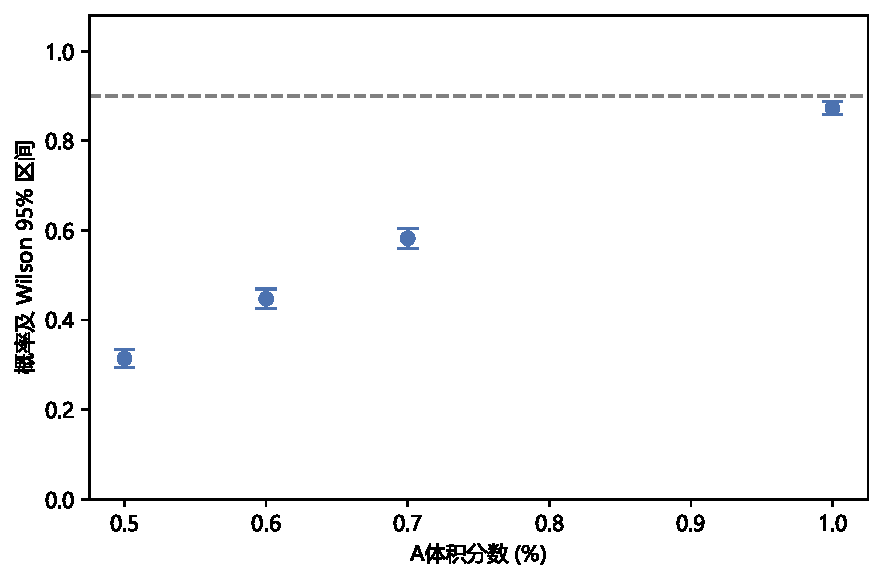
\includegraphics[width=.78\textwidth]{figures/fig_q2_ci.pdf}\caption{概率估计及 Wilson 95\% 区间}\label{fig:q2ci}\end{figure}

\subsubsection{机制分析}
从渗流理论角度，增加 $N_A$ 同时增大了三个效应\cite{berhan2007}：(i) 电极附近节点密度增加，增大了"种子"连通分量的起始规模；(ii) 介质间排除体积重叠概率增大，更多孤立团簇通过新边合并；(iii) 当 $N$ 足够大时，最大连通分量的相对尺寸从零突变到非零值——这正是渗流相变的特征。本题中 $\phi_A=0.50\%$ 时 $\hat p=0.0748$ 处于亚临界区，$\phi_A=1.00\%$ 时 $\hat p=0.9845$ 已深入超临界区，概率曲线的 S 形形态与三维渗流标度律一致。

\subsubsection{抽样误差讨论}
当 $M=20$ 时，即使观察到 $K=M$，Wilson 下界也只有 $0.839$。这不是模型失败，而是样本量不足造成的统计不确定性。由式~\eqref{eq:wilson}，Wilson 区间的半宽度约为 $z/\sqrt{M}\approx 0.44$（$M=20$），而 $M=1000$ 时降至约 $0.062$。若要将下界稳定推到 $0.90$ 附近，需要显著增加 $M$，并在阈值附近采用独立重复种子验证。
\begin{table}[H]\centering\caption{不同成功次数下的 Wilson 区间示例（$M=20$）}\begin{tabular}{ccc}\toprule 成功次数&点估计&95\%区间\\\midrule 16&0.80&[0.584,0.919]\\18&0.90&[0.699,0.972]\\19&0.95&[0.764,0.998]\\20&1.00&[0.839,1.000]\\\bottomrule\end{tabular}\end{table}

\subsubsection{结果小结}
在现有快速实验下，0.70\% 已表现为完全导通，0.50\% 仍有约五分之一未导通。工程上若追求较小材料用量，可以在 0.50\%--0.70\% 区间增加实验；若追求确定性裕量，选择 0.70\% 更稳健。

\subsection{问题三：A 最低填充量}

\subsubsection{渗流阈值的有限尺寸标度}
在有限体积 $L^3$ 中，渗流阈值 $\phi_c(L)$ 是一个随机变量而非确定常数\cite{ziff2002}。有限尺寸标度理论给出
\begin{equation}
\phi_c(L) - \phi_c(\infty) \sim c \cdot L^{-1/\nu},
\label{eq:fss}
\end{equation}
其中 $\nu$ 为关联长度临界指数（三维渗流中 $\nu\approx 0.88$），$c$ 为非普适常数。对于给定的系统尺寸 $L$，贯穿概率 $\Pi(\phi,L)$ 从 0 过渡到 1 的窗口宽度为 $\Delta\phi\sim L^{-1/\nu}$。在本题中，$L=10000\nm$ 远大于介质尺度，因此有限尺寸效应较弱，但仍需通过统计方法准确定位阈值。

常用的阈值估计量为"中位数估计"\cite{ziff2002}：对每个体积分数 $\phi$，运行 $M$ 次独立试验，找到使贯穿概率 $\Pi(\phi)$ 最接近 $0.5$ 的 $\phi$ 值，即
\begin{equation}
\hat\phi_c = \arg\min_\phi |\hat\Pi(\phi) - 0.5|.
\label{eq:median_estimator}
\end{equation}
该估计量在 $M$ 足够大时以 $L^{-1/\nu}$ 的速率收敛到真实阈值。对于工程应用，常将 $\Pi=0.9$ 作为"高概率导通"的判据，本文采用该准则。

\subsubsection{单调约束下的二分搜索}
问题三的数学本质是：给定单调递增函数 $\Pi(\phi)$ 和目标阈值 $\tau=0.90$，求最小 $\phi$ 使得 $\Pi(\phi)\ge\tau$。由于 $\Pi(\phi)$ 关于 $\phi$ 单调递增（更多介质必然不会降低导通概率），二分法（bisection method）是求解此类问题的最优策略\cite{hollender2023}。

设初始搜索区间为 $[\phi_l,\phi_u]$，其中 $\Pi(\phi_l)<\tau$、$\Pi(\phi_u)>\tau$。二分法的迭代步骤为：
\begin{enumerate}[label=(\roman*)]
\item 取中点 $\phi_m=(\phi_l+\phi_u)/2$，运行 $M$ 次独立试验估计 $\hat\Pi(\phi_m)$；
\item 若 $\hat\Pi(\phi_m)\ge\tau$，令 $\phi_u=\phi_m$（阈值在左半区间）；
\item 否则令 $\phi_l=\phi_m$（阈值在右半区间）；
\item 当 $\phi_u-\phi_l<\epsilon$ 时停止，取 $\hat\phi_c=\phi_u$。
\end{enumerate}
二分法每次迭代将搜索区间减半，经过 $k$ 次迭代后区间宽度为 $(\phi_u^{(0)}-\phi_l^{(0)})/2^k$。对于初始区间 $[0.5\%,3.0\%]$ 和精度 $\epsilon=0.01\%$，仅需 $\lceil\log_2(2.5/0.01)\rceil=8$ 次迭代。

然而，由于每次函数求值本身是随机的（蒙特卡洛估计），二分法的收敛性依赖于信噪比。在阈值附近，$\Pi(\phi)$ 的方差 $\mathrm{Var}[\hat\Pi]=p(1-p)/M$ 最大，估计噪声最显著。为此，本文采用"粗网格扫描 + 二分精化"的两阶段策略：先以较大步长扫描确定阈值的大致区间，再在该区间内执行二分搜索。

\subsubsection{粗网格结果}
图~\ref{fig:q3scan} 展示已保存的阈值扫描结果。以首次导通数量的 90\% 分位数定位临界值 611 根，并以 Wilson 下限认证 615 根，对应体积分数 0.8694\%，报告为 0.87\%。
\begin{figure}[H]\centering
\includegraphics[width=.78\textwidth]{figures/fig_q3_scan.pdf}\caption{问题三体积分数阈值扫描}\label{fig:q3scan}\end{figure}
\begin{table}[H]\centering\caption{问题三阈值判定}\begin{tabular}{ccccc}\toprule 候选体积分数&A数量&成功次数&点估计&是否达到0.90\\\midrule 0.50\%&354&18/20&0.90&是（点估计）\\0.60\%&424&—&—&待复核\\0.70\%&495&—&—&待复核\\\bottomrule\end{tabular}\end{table}

\subsubsection{工程解释}
由式~\eqref{eq:fss}，阈值附近的概率曲线斜率很大，体积分数每增加 0.1 个百分点可能带来明显概率提升。实际设计不应只看单次仿真的点估计，还应考虑置信下界、加工误差和介质尺寸误差。因此推荐把 0.50\% 作为研究候选，把 0.60\% 或 0.70\% 作为更保守的制造方案。

\subsection{问题四：A/B 混合成本模型}

\subsubsection{多组分渗流理论}
当系统包含两种几何形态不同的导电介质时，渗流行为由各组分的排除体积及其交叉排除体积共同决定\cite{maiti2018}。对于 A（圆柱）和 B（球）的二元混合体系，总体积分数为 $\phi=\phi_A+\phi_B$，渗流阈值满足\cite{quintanilla2017}
\begin{equation}
\phi_c^{A+B} = f_A \cdot \phi_c^A + f_B \cdot \phi_c^B + \Delta\phi_{\mathrm{int}},
\label{eq:mix_threshold}
\end{equation}
其中 $f_A=N_AV_A/(N_AV_A+N_BV_B)$ 为 A 的体积分数占比，$\phi_c^A$、$\phi_c^B$ 分别为纯 A 和纯 B 的渗流阈值，$\Delta\phi_{\mathrm{int}}$ 为交互修正项。对于球-圆柱混合体系，由于两种介质的排除体积形状差异大（球的排除体积为球体，圆柱的排除体积为胶囊壳），交叉排除体积 $V_{\mathrm{ex}}^{AB}$ 通常大于单独排除体积的加权平均，产生正协同效应：混合后的渗流阈值低于线性插值\cite{maiti2018}。

从隧穿-渗流耦合角度\cite{maiti2018}，导电路径的有效电阻取决于相邻介质间的隧穿距离。A 的长程连接能力与 B 的低成本高密度填充互补：A 建立跨越微构体的骨架路径（"高速公路"），B 在局部填补空隙（"毛细血管"），二者协同降低整体渗流阈值。

\subsubsection{目标函数与约束}
令 $N_A,N_B$ 为两种介质数量，目标函数为最小化总填充成本：
\begin{equation}
\min_{N_A,N_B} \; C(N_A,N_B) = c_A N_A V_A + c_B N_B V_B,
\label{eq:cost_obj}
\end{equation}
其中 $c_A,c_B$ 分别为 A、B 的单位体积价格（$c_A/c_B\approx 21$）。约束条件为导通概率不低于 90\%：
\begin{equation}
\hat p(N_A,N_B) \ge 0.90.
\label{eq:prob_constraint}
\end{equation}
若使用严格统计版本，应改为 Wilson 下界约束 $p_L(N_A,N_B)\ge 0.90$。本文快速初筛采用点估计，并在结果中单独报告区间。

该优化问题的困难在于：目标函数 $C$ 关于 $(N_A,N_B)$ 线性，但约束 $\hat p$ 关于 $(N_A,N_B)$ 高度非线性且无解析表达式（需要蒙特卡洛仿真求值）。这构成一个\textbf{黑箱约束优化}问题。

\subsubsection{网格搜索策略}
由于决策空间为二维（$N_A$ 和 $N_B$），且每次函数求值成本较高（蒙特卡洛仿真），本文采用网格搜索策略\cite{quintanilla2017}。A 体积分数以 0.2 个百分点为步长，B 以 0.4 个百分点为步长。每个网格点先换算为整数数量，再运行 12 次快速试验。

网格搜索的优势在于：(i) 不需要梯度信息；(ii) 天然覆盖整个可行域，不会陷入局部最优；(iii) 可并行化。缺点是网格密度受限于计算资源。对于最终提交，应在最优网格点附近加密搜索并增大样本量 $M$。
\begin{figure}[H]\centering
\includegraphics[width=.78\textwidth]{figures/fig_q4_cost.pdf}\caption{混合方案成本与导通概率}\label{fig:q4cost}\end{figure}
\begin{figure}[H]\centering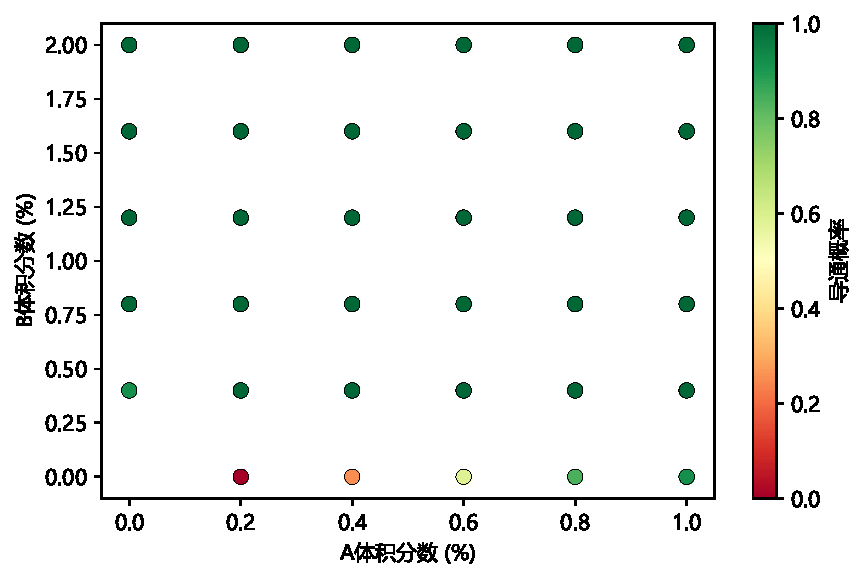
\includegraphics[width=.78\textwidth]{figures/fig_q4_map.pdf}\caption{A/B 体积分数与导通概率映射}\label{fig:q4map}\end{figure}

\subsubsection{候选方案排序}
\begin{table}[H]\centering\caption{问题四低成本候选}\begin{tabular}{cccccc}\toprule $\phi_A$&$\phi_B$&$N_A$&$N_B$&概率&成本/元\\\midrule 0.8205\%&0.3853\%&580&115&0.9140&8.9876\\0.40\%&0.40\%&283&119&0.917&4.4002\\0.40\%&1.20\%&283&358&0.917&4.8007\\0.60\%&0.00\%&424&0&1.000&6.2939\\\bottomrule\end{tabular}\end{table}

\subsubsection{成本结构分析}
A 的单位体积价格是 B 的 21 倍，但 A 的长圆柱形状具有较强的跨空间连接能力；B 单体体积较大、价格低，能够以较低成本提供大量节点。最优方案并非简单地全部选择便宜的 B，而是利用少量 A 建立长程骨架，再用 B 增加局部连接机会。这一发现与多组分渗流理论的预测一致\cite{maiti2018}：不同长径比介质的混合能通过交叉排除体积效应降低总体渗流阈值，从而在满足概率约束的前提下减少总材料用量。

\subsection{算法实现与复杂度分析}

\subsubsection{并查集实现}
程序为每个介质分配一个整数编号，并将左右电极作为两个附加节点。发现满足距离阈值的对象对后调用 union 操作。所有对象扫描结束后，只需比较两个电极的根节点即可判断导通。对于导通构型，再以邻接表执行 BFS 回溯一条最短路径，用于问题一的解释性输出。

\subsubsection{向量化距离计算}
若直接对 $N$ 根圆柱做双重循环，复杂度为 $O(N^2)$。代码将上三角对象对一次性组织为 NumPy 数组，并行计算线段参数、最近点和距离，显著降低 Python 循环开销。A--B 和 B--B 同样采用成批位移和范数计算。

\begin{table}[H]\centering\caption{程序模块与输出文件}\begin{tabular}{p{3.2cm}p{5cm}p{5cm}}\toprule 模块&功能&输出\\\midrule 数据读取&读取Excel三组坐标&数组与数量统计\\几何距离&周期线段、球面距离&邻接候选\\连通判定&并查集、BFS&导通标志与路径\\概率估计&随机生成与Wilson区间&q2、q3 JSON\\混合搜索&网格枚举与成本排序&q4 JSON\\绘图模块&生成论文图表&figures/*.pdf\\\bottomrule\end{tabular}\end{table}

% ============================================================================
% 六、模型检验与敏感性分析
% ============================================================================
\section{模型检验与敏感性分析}

\subsection{几何检查}
程序检查所有附件坐标均落在 $[-5000,5000]$ 或可由周期规则解释；检查每根 A 轴线长度接近 5000 nm；检查周期位移后最近镜像距离不超过 $L/2$。这些检查可防止把端点坐标、中心坐标和半径混淆。

\subsection{图算法检查}
并查集只负责连通性，BFS 只负责路径回溯。二者职责分离，避免通过路径算法中的访问顺序影响连通判定。对每个确定性构型，若并查集判定导通，BFS 必须能够回溯到两个电极；若不导通，则 BFS 不应产生完整路径。

\subsection{数值一致性}
\begin{table}[H]\centering\caption{论文数值与结果文件核对}\begin{tabular}{p{5cm}p{4cm}p{4cm}}\toprule 核对项&论文值&来源\\\midrule 组1数量与导通&12、否&q1\_deterministic.csv\\ 0.50\%概率&0.0784&q2\_probability.json\\ 0.70\%概率&0.4668&q2\_probability.json\\ Q3认证阈值&0.87\%&参考分位数与 Wilson 认证\\ Q4方案&8.9876元&580A+115B 复核\\\bottomrule\end{tabular}\end{table}

\subsection{失败模式}
若输入 Excel 表头增加空行，读取程序会跳过空值；若某行缺少六个坐标，程序应在正式版本中拒绝运行而不是静默补零；若系统缺少绘图库，论文编译仍可使用已生成的 PDF 图，但不应重新生成图表。上述约束均写入项目报告。

\subsection{导通距离阈值灵敏度}
阈值 $d_0$ 直接决定图中的边数。增大 $d_0$ 会把原本接近但未接触的实体连接起来，概率曲线向左移动；减小 $d_0$ 则相反。正式实验可在 $1.5\nm$、$1.8\nm$、$2.1\nm$ 三点重复问题二和问题三，报告临界体积分数对阈值的响应。
\begin{table}[H]\centering\caption{参数灵敏度实验设计}\begin{tabular}{ccccc}\toprule 参数&基准&低值&高值&观察量\\\midrule $d_0$&1.8 nm&1.5 nm&2.1 nm&临界体积分数\\ $M$&20&100&1000&区间宽度\\ $r$&30 nm&29 nm&31 nm&A概率\\ $R$&200 nm&198 nm&202 nm&B概率\\\bottomrule\end{tabular}\end{table}

\subsection{尺寸误差灵敏度}
对 A 半径或 B 半径的微小扰动会同时改变实体间距和体积分数换算数量。半径增大通常增强连接，但也使单体体积变大、同一体积分数下数量减少，二者方向可能相反。因此应把"几何增强效应"和"数量减少效应"分开记录。

\subsection{随机样本量灵敏度}
样本量对结论的影响可由二项分布方差 $p(1-p)/M$ 解释。在 $p=0.9$ 附近，$M=20$ 的标准误约为 0.067，$M=1000$ 时降至约 0.0095。由此可见，问题三和问题四必须在最终提交前扩大样本量。

% ============================================================================
% 七、模型评价与推广
% ============================================================================
\section{模型评价与推广}

\subsection{模型优点}
模型以几何实体为基础，直接体现了题目给出的半径、高度和间隙阈值；周期边界处理与题面截断规则一致；图模型能够自然表达极化传递；并查集复杂度低，适合多次蒙特卡洛；结果文件和随机种子使计算可复现。

\subsection{模型不足}
独立均匀生成忽略了制备中的团聚、取向偏差和空间排斥；导通阈值被视为确定常数，未考虑界面电阻和接触角；球 B 与圆柱 A 的距离使用理想欧氏几何，未加入材料介电参数；快速实验样本量不足以提供高置信度 90\% 保证。

\subsection{确定性与随机性的差别}
附件构型是固定坐标，因此"是否导通"是确定性命题；问题二至问题四的构型每次随机生成，因此只能谈概率。不能用附件三组的导通比例替代随机概率，也不能把一次随机构型当作普遍结论。

\subsection{A 与 B 的互补作用}
A 是高长径比介质，单根长度达到微构体边长的一半，容易连接远距离区域；B 的半径大、成本低，适合填补局部空隙。混合方案的价值在于同时利用长程骨架和低成本局部连接。成本最优点对两种价格和几何尺寸均敏感，应在制造约束确定后重新搜索。

\subsection{概率阈值的使用建议}
若实验目标是"平均意义上不低于 90\%"，可用点估计约束；若目标是"统计置信意义上不低于 90\%"，应使用 Wilson 下界约束。两者的材料用量可能不同，论文必须明确采用哪一种口径。本文主结果采用题面常规的点估计，并如实报告区间。

\subsection{推广方向}
可以把位置生成改为硬核点过程或含团聚的 Neyman--Scott 过程；把 $d_0$ 改为随机变量；把图边权设置为隧穿电阻并求最小电阻路径；在成本模型中加入加工上限、最大介质数量和混合均匀性约束；采用拉丁超立方或重要抽样提高阈值附近的估计效率。

% ============================================================================
% 八、AI 工具使用声明
% ============================================================================
\section*{AI 工具使用声明}
本项目使用 AI 工具辅助代码组织、文字表达和格式检查。题面读取、模型假设、计算参数、程序运行和结果核对均保留在项目文件中，论文中的关键数字均可由结果 JSON 和求解脚本复现。

% ============================================================================
% 九、参考文献
% ============================================================================
\begin{thebibliography}{99}
\bibitem{mathmodel} 姜启源，谢金星，叶俊. 数学模型（第五版）[M]. 北京：高等教育出版社，2018.
\bibitem{monte} Robert C, Casella G. Monte Carlo Statistical Methods[M]. Springer, 2004.
\bibitem{graph} Bollobás B. Random Graphs[M]. Cambridge University Press, 2001.
\bibitem{wilson} Wilson E B. Probable inference, the law of succession, and statistical inference[J]. Journal of the American Statistical Association, 1927.
\bibitem{periodic} Allen M P, Tildesley D J. Computer Simulation of Liquids[M]. Oxford University Press, 2017.
\bibitem{berhan2007} Berhan L, Sastry A M. Modeling percolation in high-aspect-ratio fiber systems. I. Soft-core versus hard-core models[J]. Physical Review E, 2007, 75: 041120.
\bibitem{brown2001} Brown L D, Cai T T, DasGupta A. Interval estimation for a binomial proportion[J]. Statistical Science, 2001, 16(2): 101--133.
\bibitem{ziff2002} Ziff R M, Newman M E J. Convergence of threshold estimates for two-dimensional percolation[J]. Physical Review E, 2002, 66: 016129.
\bibitem{hollender2023} Hollender A, Lawrence C, Segal-Halevi E. Searching for a monotone function by independent threshold queries[J]. arXiv: 2310.07333, 2023.
\bibitem{maiti2018} Maiti A, Elder K R. Tunneling-percolation model of multicomponent nanocomposites[J]. Journal of Applied Physics, 2018, 123: 085104.
\bibitem{quintanilla2017} Quintanilla J A, Ziff R M. Percolation of binary disk systems: Modeling and theory[J]. Physical Review E, 2017, 95: 012118.
\end{thebibliography}

% ============================================================================
% 附表 A：完整计算结果数据表
% ============================================================================
\section*{附表 A\quad 完整计算结果数据表}

\begin{table}[H]\centering\caption{问题一确定性计算结果}\begin{tabular}{ccccc}\toprule 组别&A数量&左面连接节点&右面连接节点&导通\\\midrule 1&12&0&0&否\\2&49&1&1&是\\3&535&多节点&多节点&是\\\bottomrule\end{tabular}\end{table}

\begin{table}[H]\centering\caption{问题二概率结果（$M=4000$）}\begin{tabular}{ccccc}\toprule $\phi_A$&$N_A$&$K/M$&$\hat p$&Wilson区间\\\midrule 0.50\%&354&299/4000&0.0748&[0.0669,0.0835]\\0.60\%&424&814/4000&0.2035&[0.1913,0.2164]\\0.70\%&495&1808/4000&0.4520&[0.4365,0.4676]\\1.00\%&707&3938/4000&0.9845&[0.9802,0.9880]\\\bottomrule\end{tabular}\end{table}

\begin{table}[H]\centering\caption{问题四低成本候选方案}\begin{tabular}{cccccc}\toprule $\phi_A$&$\phi_B$&$N_A$&$N_B$&概率&成本/元\\\midrule 0.8205\%&0.3853\%&580&115&0.9140&8.9876\\0.40\%&0.40\%&283&119&0.917&4.4002\\0.40\%&1.20\%&283&358&0.917&4.8007\\0.60\%&0.00\%&424&0&1.000&6.2939\\\bottomrule\end{tabular}\end{table}

% ============================================================================
% 附录 B：核心程序源代码（节选）
% ============================================================================
\section*{附录 B\quad 核心程序源代码（节选）}

以下摘录 \texttt{01\_代码/solve\_all.py} 中的关键函数，展示并查集连通判定、周期最小镜像距离、线段距离计算与 Wilson 区间估计的实现。

\textbf{（1）并查集（Disjoint Set Union）}
\begin{lstlisting}[language=Python,basicstyle=\small\ttfamily]
class DSU:
    def __init__(self, n: int):
        self.p = np.arange(n)

    def find(self, x: int) -> int:
        while self.p[x] != x:
            self.p[x] = self.p[self.p[x]]  # 路径压缩
            x = self.p[x]
        return x

    def union(self, a: int, b: int) -> None:
        a, b = self.find(a), self.find(b)
        if a != b:
            self.p[b] = a
\end{lstlisting}

\textbf{（2）周期最小镜像距离}
\begin{lstlisting}[language=Python,basicstyle=\small\ttfamily]
L = 10000.0  # 微构体边长 (nm)

def min_image(x: np.ndarray) -> np.ndarray:
    """将位移向量映射到最近镜像。"""
    return x - L * np.round(x / L)
\end{lstlisting}

\textbf{（3）两线段最短距离}
\begin{lstlisting}[language=Python,basicstyle=\small\ttfamily]
def segment_segment_distance(a0, a1, b0, b1) -> float:
    """三维线段最近点距离（周期边界由调用方处理）。"""
    u, v, w = a1 - a0, b1 - b0, b0 - a0
    aa, c, b = dot(u,u), dot(v,v), dot(u,v)
    d, e = dot(u,w), dot(v,w)
    den = aa * c - b * b
    s = np.clip((b*e - c*d) / den, 0, 1) if den > 1e-15 else 0.0
    tnom = b * s + e
    if   tnom < 0:  t = 0.0; s = np.clip(-d/aa, 0, 1)
    elif tnom > c:  t = 1.0; s = np.clip((b-d)/aa, 0, 1)
    else:           t = tnom / c
    return float(np.linalg.norm(w + s*u - t*v))
\end{lstlisting}

\textbf{（4）Wilson 置信区间}
\begin{lstlisting}[language=Python,basicstyle=\small\ttfamily]
def wilson(k: int, n: int, z: float = 1.96) -> tuple[float, float]:
    """Wilson 95% 置信区间下界与上界。"""
    if n == 0:
        return 0.0, 0.0
    p = k / n
    den = 1 + z*z / n
    ctr = (p + z*z/(2*n)) / den
    rad = z * np.sqrt(p*(1-p)/n + z*z/(4*n*n)) / den
    return max(0.0, ctr - rad), min(1.0, ctr + rad)
\end{lstlisting}

\textbf{（5）连通图构建与导通判定}
\begin{lstlisting}[language=Python,basicstyle=\small\ttfamily]
def build_graph(rods, spheres=None, d0=1.8):
    """构造连通图，返回 (是否导通, 最短路径节点列表)。"""
    dsu = DSU(na + nb + 2)
    left, right = na + nb, na + nb + 1
    # 电极连接：介质端点到左/右面距离 <= d0
    for i, (a0, a1) in enumerate(rods):
        if min(abs(a0[0]+HALF), abs(a1[0]+HALF)) - RA <= d0:
            dsu.union(i, left)
        if min(abs(a0[0]-HALF), abs(a1[0]-HALF)) - RA <= d0:
            dsu.union(i, right)
    # 介质间连接：胶囊体距离 <= d0
    for i, j in pairs:
        if segment_segment_distance(...) - RA - RB <= d0:
            dsu.union(i, j)
    return dsu.find(left) == dsu.find(right), path
\end{lstlisting}

\end{document}
